\documentclass[a4paper,12pt]{article}

\usepackage[T2A]{fontenc}
\usepackage[utf8x]{inputenc}
\usepackage[russian,english]{babel}
\usepackage{graphicx}
\usepackage{color}
\usepackage{xcolor}
\usepackage{listings}
\usepackage{fancyhdr}
\usepackage{amsmath}
\usepackage{indentfirst} % включить отступ у первого абзаца
\usepackage{array}
\usepackage{supertabular}
\usepackage{hhline}
\usepackage{semantic}

%%\usepackage[
%%		a4paper, includefoot,
%%		left=3cm, right=1cm, top=2cm, bottom=1.5cm,
%%		headsep=1cm, footskip=1cm
%%	]{geometry}

\title{Лабораторная работа №1}
\author{Кузнецов Д.Б.\and Вагин Д.А.}
\date{09/2010}
\pagestyle{empty}
\pagestyle{fancy}
\lhead{Лабораторная работа №1} %верхний колонтитул слева

\lstloadlanguages{c++,c}
\lstset{
	language=c,inputencoding=utf8x,
	extendedchars=\true,captionpos=b,tabsize=4,
	frame=lines,
	keywordstyle=\color{blue},commentstyle=\color{green},stringstyle=\color{red},
	breaklines=true,showstringspaces=false,basicstyle=\footnotesize
}

\begin{document}

\paragraph{Построение лексического анализатора на основании автоматной грамматики}
\subparagraph{Цели}
\begin{itemize}
	\item Научитсья строить лексические анализаторы на основе автоматной грамматики
\end{itemize}

\paragraph{Порядок выполнения}
\begin{enumerate}
	\item Построить автоматную грамматику
	\item Построить автомат
	\item Привести к детерминированному автомату
	\item Реализовать автомат программно на языке программирования
	\item Написать отчет
\end{enumerate}

\subparagraph{Рекомендации по выполнению}
\begin{itemize}
	\item Массивы фиксированной длины
	\item Данные задаются внутри исходного кода
\end{itemize}

\subparagraph{Состав отчета}
\begin{itemize}
	\item Титульный лист (фамилия, группа, номер варианта, наименование работы, задание)
	\item Текст задания
	\item Грамматика
	\item Диаграмма переходов
	\item Автоматы
	\item Текст программы
\end{itemize}

\paragraph{Варианты заданий}
В задании указано содержательное описание грамматики и простейши пример для облегчения понимания.
\begin{enumerate}
	\item Одинаковые символы стоят парами: $aabbaabbbbaa$
	\item В начале строки $a$: $ababbbabb$
	\item Первый символ — не важен, далее одни $a$: $baaaaaaaaa$, $aaaaaaaaaa$
	\item Либо одни $a$, либо одни $b$: $aaaaaaaaaa$, $bbbbbbbbb$
	\item В конце строки $b$: $ababbbabb$
	\item Одинаковые символы не должны стоять рядом: $ababababab$, $bababababa$
	\item В строке должна встретиться хотя бы одна буква $a$: $bbbbbabbb$, $aaaaaaaaa$
	\item Предпоследним символом строки должна быть $b$, $abbabaabb$
	\item Вторым символом строки должна быть $a$: $baaaaabbb$
	\item Два последних символа должны быть $b$: $abababb$, $bbbbbb$
	\item Первый и третий символы должны быть разными: $aabbbabab$, $baaabbbab$
	\item Первый и последний символы должны быть одинковыми: $ababababa$, $babbbabab$
\end{enumerate}

\paragraph{Пример}
\subparagraph{Задание}
Символы a и b стоят парами: abbaabab, baabbaba.
\subparagraph{Грамматика}
Построим грамматику по заданию: \\
$S -> aB$\\
$S -> bA$\\
$B -> bF$\\
$A -> aF$\\
$B -> bS$\\
$A -> aS$\\
$F -> \dashv $

\subparagraph{Автомат}
Построим диаграмму переходов \\
\centering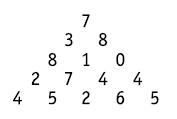
\includegraphics[scale=0.5]{images/image1.jpg}\vspace{1em}
%% TODO: сделать диаграмму на latex'е
\begin{tabular}[l]{c|cccc}
    & $-$ & $-$   & $-$   & $+$ \\
\hline
    & $S$ & $A$   & $B$   & $F$ \\
$a$ & $B$ & $S,F$ &       &     \\
$b$ & $A$ &       & $S,F$ &     \\
\end{tabular}

\subparagraph{Детерминированный автомат}
Перейдём к детерменированному автомату.\\

\begin{tabular}[l]{c|cccccc}
    & $-$ & $-$       & $-$       & $+$    & $-$    & $+$       \\
\hline
    & $S$ & $A$       & $B$       & $F$    & $\{\}$ & $\{S,F\}$ \\
$a$ & $B$ & $\{S,F\}$ &  $\{\}$   & $\{\}$ & $\{\}$ & $B$       \\
$b$ & $A$ & $\{\}$    & $\{S,F\}$ & $\{\}$ & $\{\}$ & $A$       \\
\end{tabular}

\subparagraph{Программа}
\begin{lstlisting}[language=c,{caption=анализатор}]
#include <stdio.h>

#define S  0 /* S */
#define A  1 /* A */
#define B  2 /* B */
#define F  3 /* F */
#define H  4 /* {S,F} */
#define W  5 /* {} */

#define P  1 /* + */
#define M  0 /* - */

#define a 0 /* a */
#define b 1 /* b */

struct action
{
	int sos; /* состояние */
	int out; /* вывод */
};

int main()
{
	int table[2][6];
	table[a][S] = B;
	table[b][S] = A;
	table[a][A] = H;
	table[b][A] = W;
	table[a][B] = W;
	table[b][B] = H;
	table[a][F] = W;
	table[b][F] = W;
	table[a][W] = W;
	table[b][W] = W;
	table[a][H] = B;
	table[b][H] = A;

	int output[6];
	output[S] = M;
	output[A] = M;
	output[B] = M;
	output[F] = P;
	output[W] = M;
	output[H] = P;


	int input[]={b,a,a,b};
	int n = 4, i;
	int isos = S;
 
	for( i=0; i<n; ++i)
	{
		isos=table[input[i]][isos];
	}

	printf("%d\n", output[isos]);
	return 0;
}
\end{lstlisting}

\end{document}
